% Options for packages loaded elsewhere
\PassOptionsToPackage{unicode}{hyperref}
\PassOptionsToPackage{hyphens}{url}
%
\documentclass[
]{article}
\usepackage{amsmath,amssymb}
\usepackage{iftex}
\ifPDFTeX
  \usepackage[T1]{fontenc}
  \usepackage[utf8]{inputenc}
  \usepackage{textcomp} % provide euro and other symbols
\else % if luatex or xetex
  \usepackage{unicode-math} % this also loads fontspec
  \defaultfontfeatures{Scale=MatchLowercase}
  \defaultfontfeatures[\rmfamily]{Ligatures=TeX,Scale=1}
\fi
\usepackage{lmodern}
\ifPDFTeX\else
  % xetex/luatex font selection
\fi
% Use upquote if available, for straight quotes in verbatim environments
\IfFileExists{upquote.sty}{\usepackage{upquote}}{}
\IfFileExists{microtype.sty}{% use microtype if available
  \usepackage[]{microtype}
  \UseMicrotypeSet[protrusion]{basicmath} % disable protrusion for tt fonts
}{}
\makeatletter
\@ifundefined{KOMAClassName}{% if non-KOMA class
  \IfFileExists{parskip.sty}{%
    \usepackage{parskip}
  }{% else
    \setlength{\parindent}{0pt}
    \setlength{\parskip}{6pt plus 2pt minus 1pt}}
}{% if KOMA class
  \KOMAoptions{parskip=half}}
\makeatother
\usepackage{xcolor}
\usepackage[margin=1in]{geometry}
\usepackage{color}
\usepackage{fancyvrb}
\newcommand{\VerbBar}{|}
\newcommand{\VERB}{\Verb[commandchars=\\\{\}]}
\DefineVerbatimEnvironment{Highlighting}{Verbatim}{commandchars=\\\{\}}
% Add ',fontsize=\small' for more characters per line
\usepackage{framed}
\definecolor{shadecolor}{RGB}{248,248,248}
\newenvironment{Shaded}{\begin{snugshade}}{\end{snugshade}}
\newcommand{\AlertTok}[1]{\textcolor[rgb]{0.94,0.16,0.16}{#1}}
\newcommand{\AnnotationTok}[1]{\textcolor[rgb]{0.56,0.35,0.01}{\textbf{\textit{#1}}}}
\newcommand{\AttributeTok}[1]{\textcolor[rgb]{0.13,0.29,0.53}{#1}}
\newcommand{\BaseNTok}[1]{\textcolor[rgb]{0.00,0.00,0.81}{#1}}
\newcommand{\BuiltInTok}[1]{#1}
\newcommand{\CharTok}[1]{\textcolor[rgb]{0.31,0.60,0.02}{#1}}
\newcommand{\CommentTok}[1]{\textcolor[rgb]{0.56,0.35,0.01}{\textit{#1}}}
\newcommand{\CommentVarTok}[1]{\textcolor[rgb]{0.56,0.35,0.01}{\textbf{\textit{#1}}}}
\newcommand{\ConstantTok}[1]{\textcolor[rgb]{0.56,0.35,0.01}{#1}}
\newcommand{\ControlFlowTok}[1]{\textcolor[rgb]{0.13,0.29,0.53}{\textbf{#1}}}
\newcommand{\DataTypeTok}[1]{\textcolor[rgb]{0.13,0.29,0.53}{#1}}
\newcommand{\DecValTok}[1]{\textcolor[rgb]{0.00,0.00,0.81}{#1}}
\newcommand{\DocumentationTok}[1]{\textcolor[rgb]{0.56,0.35,0.01}{\textbf{\textit{#1}}}}
\newcommand{\ErrorTok}[1]{\textcolor[rgb]{0.64,0.00,0.00}{\textbf{#1}}}
\newcommand{\ExtensionTok}[1]{#1}
\newcommand{\FloatTok}[1]{\textcolor[rgb]{0.00,0.00,0.81}{#1}}
\newcommand{\FunctionTok}[1]{\textcolor[rgb]{0.13,0.29,0.53}{\textbf{#1}}}
\newcommand{\ImportTok}[1]{#1}
\newcommand{\InformationTok}[1]{\textcolor[rgb]{0.56,0.35,0.01}{\textbf{\textit{#1}}}}
\newcommand{\KeywordTok}[1]{\textcolor[rgb]{0.13,0.29,0.53}{\textbf{#1}}}
\newcommand{\NormalTok}[1]{#1}
\newcommand{\OperatorTok}[1]{\textcolor[rgb]{0.81,0.36,0.00}{\textbf{#1}}}
\newcommand{\OtherTok}[1]{\textcolor[rgb]{0.56,0.35,0.01}{#1}}
\newcommand{\PreprocessorTok}[1]{\textcolor[rgb]{0.56,0.35,0.01}{\textit{#1}}}
\newcommand{\RegionMarkerTok}[1]{#1}
\newcommand{\SpecialCharTok}[1]{\textcolor[rgb]{0.81,0.36,0.00}{\textbf{#1}}}
\newcommand{\SpecialStringTok}[1]{\textcolor[rgb]{0.31,0.60,0.02}{#1}}
\newcommand{\StringTok}[1]{\textcolor[rgb]{0.31,0.60,0.02}{#1}}
\newcommand{\VariableTok}[1]{\textcolor[rgb]{0.00,0.00,0.00}{#1}}
\newcommand{\VerbatimStringTok}[1]{\textcolor[rgb]{0.31,0.60,0.02}{#1}}
\newcommand{\WarningTok}[1]{\textcolor[rgb]{0.56,0.35,0.01}{\textbf{\textit{#1}}}}
\usepackage{graphicx}
\makeatletter
\def\maxwidth{\ifdim\Gin@nat@width>\linewidth\linewidth\else\Gin@nat@width\fi}
\def\maxheight{\ifdim\Gin@nat@height>\textheight\textheight\else\Gin@nat@height\fi}
\makeatother
% Scale images if necessary, so that they will not overflow the page
% margins by default, and it is still possible to overwrite the defaults
% using explicit options in \includegraphics[width, height, ...]{}
\setkeys{Gin}{width=\maxwidth,height=\maxheight,keepaspectratio}
% Set default figure placement to htbp
\makeatletter
\def\fps@figure{htbp}
\makeatother
\setlength{\emergencystretch}{3em} % prevent overfull lines
\providecommand{\tightlist}{%
  \setlength{\itemsep}{0pt}\setlength{\parskip}{0pt}}
\setcounter{secnumdepth}{-\maxdimen} % remove section numbering
\ifLuaTeX
  \usepackage{selnolig}  % disable illegal ligatures
\fi
\usepackage{bookmark}
\IfFileExists{xurl.sty}{\usepackage{xurl}}{} % add URL line breaks if available
\urlstyle{same}
\hypersetup{
  pdftitle={GC measurements against MLCS measurements},
  hidelinks,
  pdfcreator={LaTeX via pandoc}}

\title{GC measurements against MLCS measurements}
\author{}
\date{\vspace{-2.5em}}

\begin{document}
\maketitle

\section{Necessary libraries}\label{necessary-libraries}

\section{Read file}\label{read-file}

\begin{Shaded}
\begin{Highlighting}[]
\NormalTok{master }\OtherTok{\textless{}{-}} \FunctionTok{read\_excel}\NormalTok{(}\StringTok{"RES \_LCMS\_GC.xlsx"}\NormalTok{, }\AttributeTok{sheet=}\DecValTok{1}\NormalTok{)}
\NormalTok{master}\SpecialCharTok{$}\NormalTok{Sensor }\OtherTok{\textless{}{-}} \FunctionTok{as.factor}\NormalTok{(master}\SpecialCharTok{$}\NormalTok{Sensor)}

\NormalTok{fan\_off }\OtherTok{\textless{}{-}}\NormalTok{ master }\SpecialCharTok{\%\textgreater{}\%} 
        \FunctionTok{select}\NormalTok{(}\SpecialCharTok{{-}}\NormalTok{LCMS\_ppm\_hr\_fan\_on, }\SpecialCharTok{{-}}\NormalTok{LCMS\_ppm\_hr\_3point)  }\SpecialCharTok{\%\textgreater{}\%} 
        \FunctionTok{na.omit}\NormalTok{()}

\NormalTok{fan\_on }\OtherTok{\textless{}{-}}\NormalTok{ master }\SpecialCharTok{\%\textgreater{}\%} 
        \FunctionTok{select}\NormalTok{(}\SpecialCharTok{{-}}\NormalTok{LCMS\_ppm\_hr, }\SpecialCharTok{{-}}\NormalTok{LCMS\_ppm\_hr\_3point)  }\SpecialCharTok{\%\textgreater{}\%} 
        \FunctionTok{na.omit}\NormalTok{()}

\NormalTok{three\_point }\OtherTok{\textless{}{-}}\NormalTok{ master }\SpecialCharTok{\%\textgreater{}\%} 
        \FunctionTok{select}\NormalTok{(}\SpecialCharTok{{-}}\NormalTok{LCMS\_ppm\_hr, }\SpecialCharTok{{-}}\NormalTok{LCMS\_ppm\_hr\_fan\_on)  }\SpecialCharTok{\%\textgreater{}\%} 
        \FunctionTok{na.omit}\NormalTok{()}

\FunctionTok{str}\NormalTok{(master)}
\end{Highlighting}
\end{Shaded}

\begin{verbatim}
## tibble [79 x 6] (S3: tbl_df/tbl/data.frame)
##  $ Plot              : chr [1:79] "C1_Vincent_Aug1" "SMW2_Vincent_Aug1" "C1_SMW2_Vincent_Aug27" "C1_Vincent_Jun27" ...
##  $ Sensor            : Factor w/ 3 levels "1","2","3": 1 1 1 1 1 3 3 2 2 2 ...
##  $ GC_ppm_hr         : num [1:79] 69.4 107.5 NA 83.1 63.2 ...
##  $ LCMS_ppm_hr       : num [1:79] 26.8 43.4 NA 25.6 33.2 ...
##  $ LCMS_ppm_hr_fan_on: num [1:79] 64.2 86.4 NA NA NA ...
##  $ LCMS_ppm_hr_3point: num [1:79] 25.6 38.8 NA 26.9 36.2 ...
\end{verbatim}

\section{fan off}\label{fan-off}

\begin{Shaded}
\begin{Highlighting}[]
\NormalTok{all\_plotted\_fan\_off }\OtherTok{\textless{}{-}}
\FunctionTok{ggplot}\NormalTok{(}\AttributeTok{data=}\NormalTok{fan\_off, }\FunctionTok{aes}\NormalTok{(}\AttributeTok{x=}\NormalTok{LCMS\_ppm\_hr, }\AttributeTok{y=}\NormalTok{GC\_ppm\_hr))}\SpecialCharTok{+}
  \FunctionTok{geom\_point}\NormalTok{(}\FunctionTok{aes}\NormalTok{(}\AttributeTok{color=}\NormalTok{Sensor))}\SpecialCharTok{+}
  \FunctionTok{scale\_x\_continuous}\NormalTok{(}\AttributeTok{limits =} \FunctionTok{c}\NormalTok{(}\SpecialCharTok{{-}}\DecValTok{0}\NormalTok{, }\DecValTok{149}\NormalTok{), }\AttributeTok{expand =} \FunctionTok{c}\NormalTok{(}\DecValTok{0}\NormalTok{, }\DecValTok{0}\NormalTok{))}\SpecialCharTok{+}
  \FunctionTok{scale\_y\_continuous}\NormalTok{(}\AttributeTok{limits =} \FunctionTok{c}\NormalTok{(}\SpecialCharTok{{-}}\DecValTok{0}\NormalTok{, }\DecValTok{149}\NormalTok{), }\AttributeTok{expand =} \FunctionTok{c}\NormalTok{(}\DecValTok{0}\NormalTok{, }\DecValTok{0}\NormalTok{))}\SpecialCharTok{+}
  \FunctionTok{geom\_abline}\NormalTok{(}\AttributeTok{intercept =} \DecValTok{0}\NormalTok{, }\AttributeTok{slope =} \DecValTok{1}\NormalTok{)}\SpecialCharTok{+}
  \FunctionTok{stat\_regline\_equation}\NormalTok{(}\FunctionTok{aes}\NormalTok{(}\AttributeTok{x=}\NormalTok{LCMS\_ppm\_hr, }\AttributeTok{y=}\NormalTok{GC\_ppm\_hr, }
    \AttributeTok{label =}  \FunctionTok{paste}\NormalTok{(..rr.label..)),}
    \AttributeTok{show.legend =} \ConstantTok{FALSE}\NormalTok{, }
    \AttributeTok{label.x =} \DecValTok{75}\NormalTok{,}
    \AttributeTok{label.y =} \DecValTok{45}\NormalTok{)}\SpecialCharTok{+}
  \FunctionTok{stat\_regline\_equation}\NormalTok{(}\FunctionTok{aes}\NormalTok{(}\AttributeTok{x=}\NormalTok{LCMS\_ppm\_hr, }\AttributeTok{y=}\NormalTok{GC\_ppm\_hr, }
    \AttributeTok{label =} \FunctionTok{paste}\NormalTok{(..eq.label..)),}
    \AttributeTok{show.legend =} \ConstantTok{FALSE}\NormalTok{, }
    \AttributeTok{label.x =} \DecValTok{75}\NormalTok{, }
    \AttributeTok{label.y =} \DecValTok{50}\NormalTok{)}\SpecialCharTok{+}
  \FunctionTok{geom\_smooth}\NormalTok{(}\AttributeTok{data=}\NormalTok{fan\_off, }\FunctionTok{aes}\NormalTok{(}\AttributeTok{x=}\NormalTok{LCMS\_ppm\_hr, }\AttributeTok{y=}\NormalTok{GC\_ppm\_hr),}\AttributeTok{method=}\StringTok{"lm"}\NormalTok{, }\AttributeTok{level =} \FloatTok{0.95}\NormalTok{)}\SpecialCharTok{+}
  \FunctionTok{ggtitle}\NormalTok{(}\StringTok{"(a) Fan off"}\NormalTok{)}
  

\NormalTok{all\_plotted\_fan\_off}
\end{Highlighting}
\end{Shaded}

\begin{verbatim}
## Warning: The dot-dot notation (`..rr.label..`) was deprecated in ggplot2 3.4.0.
## i Please use `after_stat(rr.label)` instead.
## This warning is displayed once every 8 hours.
## Call `lifecycle::last_lifecycle_warnings()` to see where this warning was
## generated.
\end{verbatim}

\begin{verbatim}
## `geom_smooth()` using formula = 'y ~ x'
\end{verbatim}

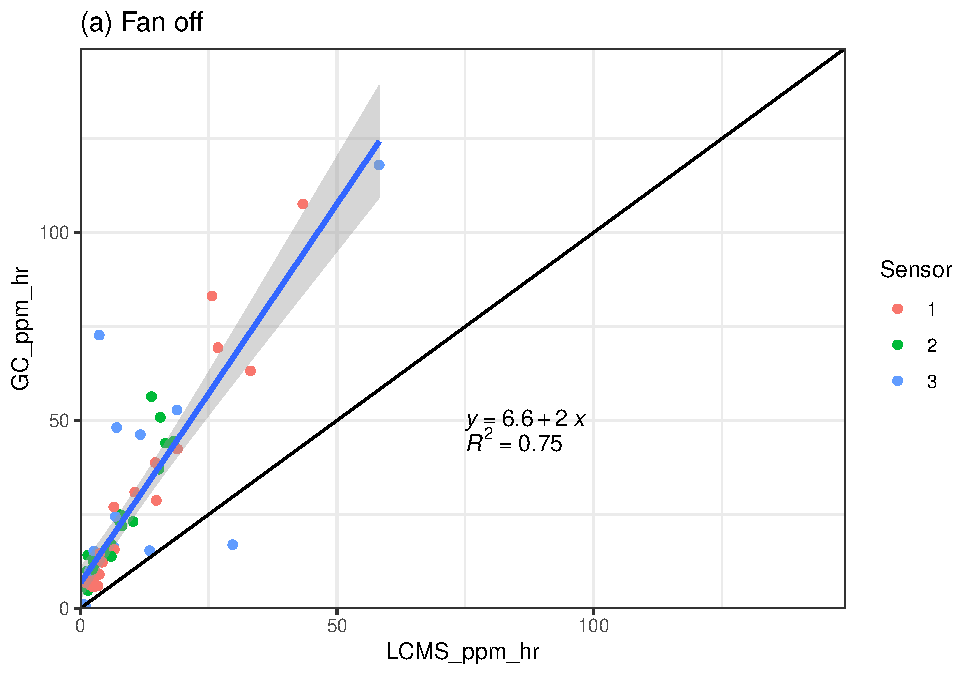
\includegraphics{Initial_look_GC_LCMS_files/figure-latex/unnamed-chunk-3-1.pdf}

\begin{Shaded}
\begin{Highlighting}[]
\FunctionTok{summary}\NormalTok{(}\FunctionTok{lm}\NormalTok{(GC\_ppm\_hr}\SpecialCharTok{\textasciitilde{}}\NormalTok{LCMS\_ppm\_hr, }\AttributeTok{data =}\NormalTok{fan\_off)) }\CommentTok{\#coefficents are the same, y=mx+c and r2}
\end{Highlighting}
\end{Shaded}

\begin{verbatim}
## 
## Call:
## lm(formula = GC_ppm_hr ~ LCMS_ppm_hr, data = fan_off)
## 
## Residuals:
##     Min      1Q  Median      3Q     Max 
## -49.645  -4.912  -1.575   2.623  58.561 
## 
## Coefficients:
##             Estimate Std. Error t value Pr(>|t|)    
## (Intercept)   6.6319     2.0679   3.207  0.00214 ** 
## LCMS_ppm_hr   2.0189     0.1478  13.660  < 2e-16 ***
## ---
## Signif. codes:  0 '***' 0.001 '**' 0.01 '*' 0.05 '.' 0.1 ' ' 1
## 
## Residual standard error: 12.68 on 61 degrees of freedom
## Multiple R-squared:  0.7536, Adjusted R-squared:  0.7496 
## F-statistic: 186.6 on 1 and 61 DF,  p-value: < 2.2e-16
\end{verbatim}

\section{fan off transformed}\label{fan-off-transformed}

\begin{Shaded}
\begin{Highlighting}[]
\NormalTok{lm\_fan\_off }\OtherTok{\textless{}{-}} \FunctionTok{lm}\NormalTok{(GC\_ppm\_hr}\SpecialCharTok{\textasciitilde{}}\NormalTok{LCMS\_ppm\_hr, }\AttributeTok{data =}\NormalTok{fan\_off)}

\NormalTok{fan\_off}\SpecialCharTok{$}\NormalTok{fan\_off\_predicted\_ppm }\OtherTok{\textless{}{-}} \FunctionTok{predict}\NormalTok{(lm\_fan\_off, fan\_off)}

\CommentTok{\#pearson\textquotesingle{}s correlation test}
\FunctionTok{cor.test}\NormalTok{(fan\_off}\SpecialCharTok{$}\NormalTok{GC\_ppm\_hr,fan\_off}\SpecialCharTok{$}\NormalTok{fan\_off\_predicted\_ppm, }\AttributeTok{method =} \StringTok{"pearson"}\NormalTok{)}
\end{Highlighting}
\end{Shaded}

\begin{verbatim}
## 
##  Pearson's product-moment correlation
## 
## data:  fan_off$GC_ppm_hr and fan_off$fan_off_predicted_ppm
## t = 13.66, df = 61, p-value < 2.2e-16
## alternative hypothesis: true correlation is not equal to 0
## 95 percent confidence interval:
##  0.7903556 0.9183577
## sample estimates:
##       cor 
## 0.8681227
\end{verbatim}

\begin{Shaded}
\begin{Highlighting}[]
\NormalTok{all\_plotted\_fan\_off\_predicted }\OtherTok{\textless{}{-}}
\FunctionTok{ggplot}\NormalTok{(}\AttributeTok{data=}\NormalTok{fan\_off, }\FunctionTok{aes}\NormalTok{(}\AttributeTok{x=}\NormalTok{fan\_off\_predicted\_ppm, }\AttributeTok{y=}\NormalTok{GC\_ppm\_hr))}\SpecialCharTok{+}
  \FunctionTok{geom\_point}\NormalTok{(}\FunctionTok{aes}\NormalTok{(}\AttributeTok{color=}\NormalTok{Sensor))}\SpecialCharTok{+}
  \FunctionTok{scale\_x\_continuous}\NormalTok{(}\AttributeTok{limits =} \FunctionTok{c}\NormalTok{(}\SpecialCharTok{{-}}\DecValTok{0}\NormalTok{, }\DecValTok{149}\NormalTok{), }\AttributeTok{expand =} \FunctionTok{c}\NormalTok{(}\DecValTok{0}\NormalTok{, }\DecValTok{0}\NormalTok{))}\SpecialCharTok{+}
  \FunctionTok{scale\_y\_continuous}\NormalTok{(}\AttributeTok{limits =} \FunctionTok{c}\NormalTok{(}\SpecialCharTok{{-}}\DecValTok{0}\NormalTok{, }\DecValTok{149}\NormalTok{), }\AttributeTok{expand =} \FunctionTok{c}\NormalTok{(}\DecValTok{0}\NormalTok{, }\DecValTok{0}\NormalTok{))}\SpecialCharTok{+}
  \FunctionTok{geom\_abline}\NormalTok{(}\AttributeTok{intercept =} \DecValTok{0}\NormalTok{, }\AttributeTok{slope =} \DecValTok{1}\NormalTok{)}\SpecialCharTok{+}
  \FunctionTok{geom\_smooth}\NormalTok{(}\AttributeTok{data=}\NormalTok{fan\_off, }\FunctionTok{aes}\NormalTok{(}\AttributeTok{x=}\NormalTok{fan\_off\_predicted\_ppm, }\AttributeTok{y=}\NormalTok{GC\_ppm\_hr),}\AttributeTok{method=}\StringTok{"lm"}\NormalTok{, }\AttributeTok{level =} \FloatTok{0.95}\NormalTok{)}\SpecialCharTok{+}
  \FunctionTok{ggtitle}\NormalTok{(}\StringTok{"(b) Fan off predicted"}\NormalTok{)}\SpecialCharTok{+}
  \FunctionTok{annotate}\NormalTok{(}\StringTok{"text"}\NormalTok{, }\AttributeTok{x=}\DecValTok{50}\NormalTok{, }\AttributeTok{y=}\DecValTok{100}\NormalTok{, }
           \AttributeTok{label =} \FunctionTok{paste}\NormalTok{(}\StringTok{"Pearson\textquotesingle{}s Correlation ="}\NormalTok{, }
                         \FunctionTok{round}\NormalTok{(}\FunctionTok{cor}\NormalTok{(fan\_off}\SpecialCharTok{$}\NormalTok{GC\_ppm\_hr, fan\_off}\SpecialCharTok{$}\NormalTok{fan\_off\_predicted\_ppm, }\AttributeTok{method =} \StringTok{"pearson"}\NormalTok{), }\DecValTok{2}\NormalTok{)))}
\end{Highlighting}
\end{Shaded}

\section{fan off histogram}\label{fan-off-histogram}

\begin{Shaded}
\begin{Highlighting}[]
\NormalTok{fan\_off}\SpecialCharTok{$}\NormalTok{diff }\OtherTok{\textless{}{-}}\NormalTok{ fan\_off}\SpecialCharTok{$}\NormalTok{fan\_off\_predicted\_ppm }\SpecialCharTok{{-}}\NormalTok{ fan\_off}\SpecialCharTok{$}\NormalTok{GC\_ppm\_hr}

\NormalTok{center\_value\_fan\_off }\OtherTok{\textless{}{-}} \FunctionTok{median}\NormalTok{(fan\_off}\SpecialCharTok{$}\NormalTok{diff)  }\CommentTok{\# Find the center of the histogram}

\NormalTok{fan\_off\_histogram }\OtherTok{\textless{}{-}}
\FunctionTok{ggplot}\NormalTok{(fan\_off, }\FunctionTok{aes}\NormalTok{(}\AttributeTok{x =}\NormalTok{ diff)) }\SpecialCharTok{+} 
  \FunctionTok{geom\_histogram}\NormalTok{(}\AttributeTok{binwidth =} \DecValTok{1}\NormalTok{, }\AttributeTok{fill =} \StringTok{"skyblue"}\NormalTok{, }\AttributeTok{color =} \StringTok{"black"}\NormalTok{) }\SpecialCharTok{+}
  \FunctionTok{labs}\NormalTok{(}
    \AttributeTok{x =} \StringTok{"Difference in ΔC (ppm/hr, predicted MLCS {-} GC)"}\NormalTok{,  }\CommentTok{\# Rename x{-}axis}
    \AttributeTok{y =} \StringTok{"Frequency"}
\NormalTok{  ) }\SpecialCharTok{+}
  \FunctionTok{scale\_x\_continuous}\NormalTok{(}\AttributeTok{breaks =} \FunctionTok{c}\NormalTok{(}\FunctionTok{round}\NormalTok{(center\_value\_fan\_off, }\DecValTok{2}\NormalTok{), }\DecValTok{30}\NormalTok{, }\SpecialCharTok{{-}}\DecValTok{30}\NormalTok{,}\SpecialCharTok{{-}}\DecValTok{60}\NormalTok{,}\DecValTok{60}\NormalTok{), }\AttributeTok{limits =} \FunctionTok{c}\NormalTok{(}\SpecialCharTok{{-}}\DecValTok{60}\NormalTok{,}\DecValTok{60}\NormalTok{))}\SpecialCharTok{+}
  \FunctionTok{geom\_vline}\NormalTok{(}\AttributeTok{xintercept =}\NormalTok{ center\_value\_fan\_off, }\AttributeTok{linetype =} \StringTok{"dashed"}\NormalTok{, }\AttributeTok{color =} \StringTok{"red"}\NormalTok{, }\AttributeTok{size =} \FloatTok{1.5}\NormalTok{)}\SpecialCharTok{+}
  \FunctionTok{theme\_minimal}\NormalTok{()}\SpecialCharTok{+}
  \FunctionTok{ggtitle}\NormalTok{(}\StringTok{"(c) Fan off: Difference distribution"}\NormalTok{)}
\end{Highlighting}
\end{Shaded}

\begin{verbatim}
## Warning: Using `size` aesthetic for lines was deprecated in ggplot2 3.4.0.
## i Please use `linewidth` instead.
## This warning is displayed once every 8 hours.
## Call `lifecycle::last_lifecycle_warnings()` to see where this warning was
## generated.
\end{verbatim}

\begin{Shaded}
\begin{Highlighting}[]
\FunctionTok{cor.test}\NormalTok{(fan\_off}\SpecialCharTok{$}\NormalTok{GC\_ppm\_hr,fan\_off}\SpecialCharTok{$}\NormalTok{fan\_off\_predicted\_ppm, }\AttributeTok{method =} \StringTok{"pearson"}\NormalTok{)}
\end{Highlighting}
\end{Shaded}

\begin{verbatim}
## 
##  Pearson's product-moment correlation
## 
## data:  fan_off$GC_ppm_hr and fan_off$fan_off_predicted_ppm
## t = 13.66, df = 61, p-value < 2.2e-16
## alternative hypothesis: true correlation is not equal to 0
## 95 percent confidence interval:
##  0.7903556 0.9183577
## sample estimates:
##       cor 
## 0.8681227
\end{verbatim}

\section{fan on}\label{fan-on}

\begin{Shaded}
\begin{Highlighting}[]
\NormalTok{all\_plotted\_fan\_on }\OtherTok{\textless{}{-}}
\FunctionTok{ggplot}\NormalTok{(}\AttributeTok{data=}\NormalTok{fan\_on, }\FunctionTok{aes}\NormalTok{(}\AttributeTok{x=}\NormalTok{LCMS\_ppm\_hr\_fan\_on, }\AttributeTok{y=}\NormalTok{GC\_ppm\_hr))}\SpecialCharTok{+}
  \FunctionTok{geom\_point}\NormalTok{(}\FunctionTok{aes}\NormalTok{(}\AttributeTok{color=}\NormalTok{Sensor))}\SpecialCharTok{+}
  \FunctionTok{scale\_x\_continuous}\NormalTok{(}\AttributeTok{limits =} \FunctionTok{c}\NormalTok{(}\SpecialCharTok{{-}}\DecValTok{0}\NormalTok{, }\DecValTok{149}\NormalTok{), }\AttributeTok{expand =} \FunctionTok{c}\NormalTok{(}\DecValTok{0}\NormalTok{, }\DecValTok{0}\NormalTok{))}\SpecialCharTok{+}
  \FunctionTok{scale\_y\_continuous}\NormalTok{(}\AttributeTok{limits =} \FunctionTok{c}\NormalTok{(}\SpecialCharTok{{-}}\DecValTok{0}\NormalTok{, }\DecValTok{149}\NormalTok{), }\AttributeTok{expand =} \FunctionTok{c}\NormalTok{(}\DecValTok{0}\NormalTok{, }\DecValTok{0}\NormalTok{))}\SpecialCharTok{+}
  \FunctionTok{geom\_abline}\NormalTok{(}\AttributeTok{intercept =} \DecValTok{0}\NormalTok{, }\AttributeTok{slope =} \DecValTok{1}\NormalTok{)}\SpecialCharTok{+}
  \FunctionTok{stat\_regline\_equation}\NormalTok{(}\FunctionTok{aes}\NormalTok{(}\AttributeTok{x=}\NormalTok{LCMS\_ppm\_hr\_fan\_on, }\AttributeTok{y=}\NormalTok{GC\_ppm\_hr, }
    \AttributeTok{label =}  \FunctionTok{paste}\NormalTok{(..rr.label..)),}
    \AttributeTok{show.legend =} \ConstantTok{FALSE}\NormalTok{, }
    \AttributeTok{label.x =} \DecValTok{75}\NormalTok{,}
    \AttributeTok{label.y =} \DecValTok{45}\NormalTok{)}\SpecialCharTok{+}
  \FunctionTok{stat\_regline\_equation}\NormalTok{(}\FunctionTok{aes}\NormalTok{(}\AttributeTok{x=}\NormalTok{LCMS\_ppm\_hr\_fan\_on, }\AttributeTok{y=}\NormalTok{GC\_ppm\_hr, }
    \AttributeTok{label =} \FunctionTok{paste}\NormalTok{(..eq.label..)),}
    \AttributeTok{show.legend =} \ConstantTok{FALSE}\NormalTok{, }
    \AttributeTok{label.x =} \DecValTok{75}\NormalTok{, }
    \AttributeTok{label.y =} \DecValTok{50}\NormalTok{)}\SpecialCharTok{+}
  \FunctionTok{geom\_smooth}\NormalTok{(}\AttributeTok{data=}\NormalTok{fan\_on, }\FunctionTok{aes}\NormalTok{(}\AttributeTok{x=}\NormalTok{LCMS\_ppm\_hr\_fan\_on, }\AttributeTok{y=}\NormalTok{GC\_ppm\_hr),}\AttributeTok{method=}\StringTok{"lm"}\NormalTok{, }\AttributeTok{level =} \FloatTok{0.95}\NormalTok{)}\SpecialCharTok{+}
  \FunctionTok{ggtitle}\NormalTok{(}\StringTok{"Fan on"}\NormalTok{)}\SpecialCharTok{+}
  \FunctionTok{theme}\NormalTok{(}\AttributeTok{legend.position=}\StringTok{"bottom"}\NormalTok{)}\SpecialCharTok{+}
  \FunctionTok{annotate}\NormalTok{(}\StringTok{"text"}\NormalTok{, }\AttributeTok{x=}\DecValTok{30}\NormalTok{, }\AttributeTok{y=}\DecValTok{100}\NormalTok{, }
           \AttributeTok{label =} \FunctionTok{paste}\NormalTok{(}\StringTok{"Pearson\textquotesingle{}s Correlation ="}\NormalTok{, }
                         \FunctionTok{round}\NormalTok{(}\FunctionTok{cor}\NormalTok{(fan\_on}\SpecialCharTok{$}\NormalTok{GC\_ppm\_hr, fan\_on}\SpecialCharTok{$}\NormalTok{LCMS\_ppm\_hr\_fan\_on, }\AttributeTok{method =} \StringTok{"pearson"}\NormalTok{), }\DecValTok{2}\NormalTok{)))}
  

\NormalTok{all\_plotted\_fan\_on}
\end{Highlighting}
\end{Shaded}

\begin{verbatim}
## `geom_smooth()` using formula = 'y ~ x'
\end{verbatim}

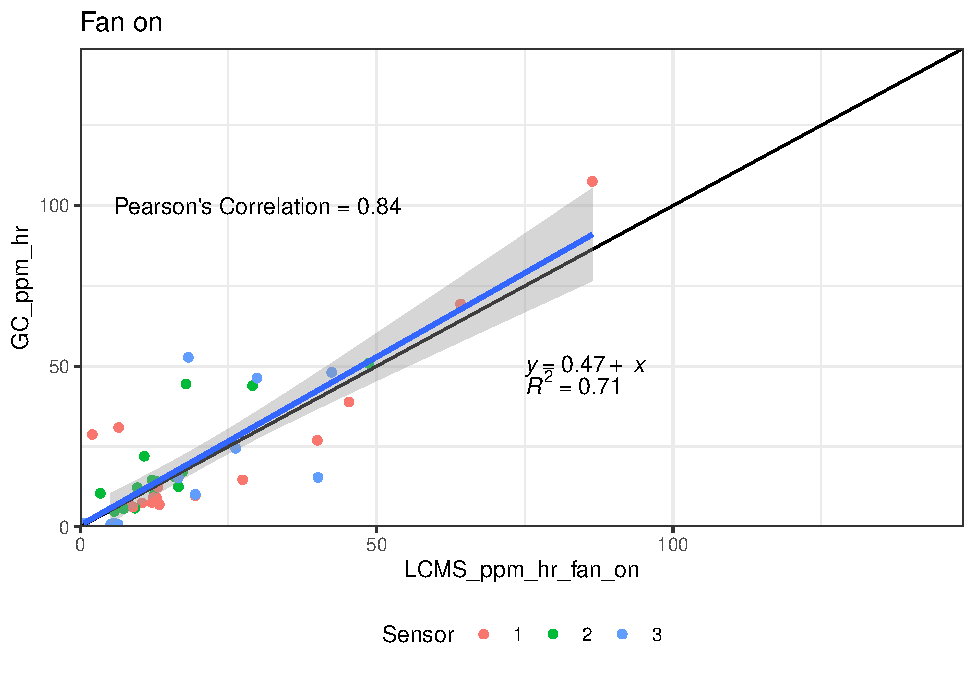
\includegraphics{Initial_look_GC_LCMS_files/figure-latex/unnamed-chunk-6-1.pdf}

\begin{Shaded}
\begin{Highlighting}[]
\FunctionTok{summary}\NormalTok{(}\FunctionTok{lm}\NormalTok{(GC\_ppm\_hr}\SpecialCharTok{\textasciitilde{}}\NormalTok{LCMS\_ppm\_hr\_fan\_on, }\AttributeTok{data =}\NormalTok{fan\_on)) }\CommentTok{\#coefficents are the same, y=mx+c and r2}
\end{Highlighting}
\end{Shaded}

\begin{verbatim}
## 
## Call:
## lm(formula = GC_ppm_hr ~ LCMS_ppm_hr_fan_on, data = fan_on)
## 
## Residuals:
##     Min      1Q  Median      3Q     Max 
## -27.096  -5.367  -2.521   1.643  33.215 
## 
## Coefficients:
##                    Estimate Std. Error t value Pr(>|t|)    
## (Intercept)          0.4735     2.6207   0.181    0.857    
## LCMS_ppm_hr_fan_on   1.0477     0.1024  10.236 5.57e-13 ***
## ---
## Signif. codes:  0 '***' 0.001 '**' 0.01 '*' 0.05 '.' 0.1 ' ' 1
## 
## Residual standard error: 11.68 on 42 degrees of freedom
## Multiple R-squared:  0.7138, Adjusted R-squared:  0.707 
## F-statistic: 104.8 on 1 and 42 DF,  p-value: 5.567e-13
\end{verbatim}

\begin{Shaded}
\begin{Highlighting}[]
\FunctionTok{cor.test}\NormalTok{(fan\_on}\SpecialCharTok{$}\NormalTok{GC\_ppm\_hr,fan\_on}\SpecialCharTok{$}\NormalTok{LCMS\_ppm\_hr\_fan\_on, }\AttributeTok{method =} \StringTok{"pearson"}\NormalTok{)}
\end{Highlighting}
\end{Shaded}

\begin{verbatim}
## 
##  Pearson's product-moment correlation
## 
## data:  fan_on$GC_ppm_hr and fan_on$LCMS_ppm_hr_fan_on
## t = 10.236, df = 42, p-value = 5.567e-13
## alternative hypothesis: true correlation is not equal to 0
## 95 percent confidence interval:
##  0.7314985 0.9128122
## sample estimates:
##       cor 
## 0.8448951
\end{verbatim}

\section{three point}\label{three-point}

\begin{Shaded}
\begin{Highlighting}[]
\NormalTok{all\_plotted\_three\_point }\OtherTok{\textless{}{-}}
\FunctionTok{ggplot}\NormalTok{(}\AttributeTok{data=}\NormalTok{three\_point, }\FunctionTok{aes}\NormalTok{(}\AttributeTok{x=}\NormalTok{LCMS\_ppm\_hr\_3point, }\AttributeTok{y=}\NormalTok{GC\_ppm\_hr))}\SpecialCharTok{+}
  \FunctionTok{geom\_point}\NormalTok{(}\FunctionTok{aes}\NormalTok{(}\AttributeTok{color=}\NormalTok{Sensor))}\SpecialCharTok{+}
  \FunctionTok{scale\_x\_continuous}\NormalTok{(}\AttributeTok{limits =} \FunctionTok{c}\NormalTok{(}\SpecialCharTok{{-}}\DecValTok{0}\NormalTok{, }\DecValTok{149}\NormalTok{), }\AttributeTok{expand =} \FunctionTok{c}\NormalTok{(}\DecValTok{0}\NormalTok{, }\DecValTok{0}\NormalTok{))}\SpecialCharTok{+}
  \FunctionTok{scale\_y\_continuous}\NormalTok{(}\AttributeTok{limits =} \FunctionTok{c}\NormalTok{(}\SpecialCharTok{{-}}\DecValTok{0}\NormalTok{, }\DecValTok{149}\NormalTok{), }\AttributeTok{expand =} \FunctionTok{c}\NormalTok{(}\DecValTok{0}\NormalTok{, }\DecValTok{0}\NormalTok{))}\SpecialCharTok{+}
  \FunctionTok{geom\_abline}\NormalTok{(}\AttributeTok{intercept =} \DecValTok{0}\NormalTok{, }\AttributeTok{slope =} \DecValTok{1}\NormalTok{)}\SpecialCharTok{+}
  \FunctionTok{stat\_regline\_equation}\NormalTok{(}\FunctionTok{aes}\NormalTok{(}\AttributeTok{x=}\NormalTok{LCMS\_ppm\_hr\_3point, }\AttributeTok{y=}\NormalTok{GC\_ppm\_hr, }
    \AttributeTok{label =}  \FunctionTok{paste}\NormalTok{(..rr.label..)),}
    \AttributeTok{show.legend =} \ConstantTok{FALSE}\NormalTok{, }
    \AttributeTok{label.x =} \DecValTok{75}\NormalTok{,}
    \AttributeTok{label.y =} \DecValTok{45}\NormalTok{)}\SpecialCharTok{+}
  \FunctionTok{stat\_regline\_equation}\NormalTok{(}\FunctionTok{aes}\NormalTok{(}\AttributeTok{x=}\NormalTok{LCMS\_ppm\_hr\_3point, }\AttributeTok{y=}\NormalTok{GC\_ppm\_hr, }
    \AttributeTok{label =} \FunctionTok{paste}\NormalTok{(..eq.label..)),}
    \AttributeTok{show.legend =} \ConstantTok{FALSE}\NormalTok{, }
    \AttributeTok{label.x =} \DecValTok{75}\NormalTok{, }
    \AttributeTok{label.y =} \DecValTok{50}\NormalTok{)}\SpecialCharTok{+}
  \FunctionTok{geom\_smooth}\NormalTok{(}\AttributeTok{data=}\NormalTok{three\_point, }\FunctionTok{aes}\NormalTok{(}\AttributeTok{x=}\NormalTok{LCMS\_ppm\_hr\_3point, }\AttributeTok{y=}\NormalTok{GC\_ppm\_hr),}\AttributeTok{method=}\StringTok{"lm"}\NormalTok{, }\AttributeTok{level =} \FloatTok{0.95}\NormalTok{)}\SpecialCharTok{+}
  \FunctionTok{ggtitle}\NormalTok{(}\StringTok{"(d) Three point"}\NormalTok{)}
  

\NormalTok{all\_plotted\_three\_point}
\end{Highlighting}
\end{Shaded}

\begin{verbatim}
## `geom_smooth()` using formula = 'y ~ x'
\end{verbatim}

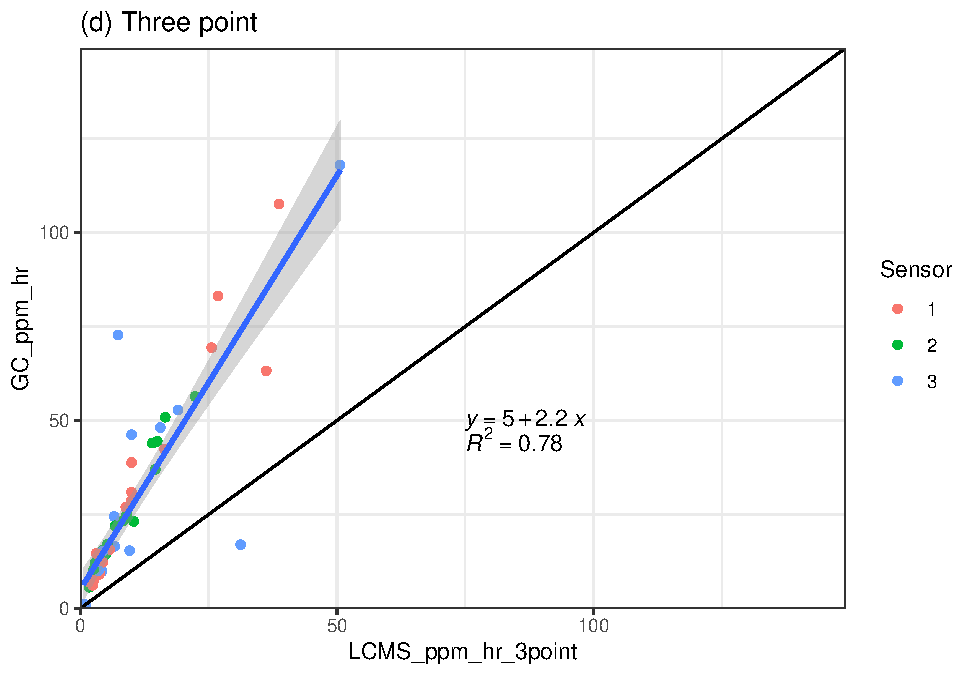
\includegraphics{Initial_look_GC_LCMS_files/figure-latex/unnamed-chunk-7-1.pdf}

\begin{Shaded}
\begin{Highlighting}[]
\FunctionTok{summary}\NormalTok{(}\FunctionTok{lm}\NormalTok{(GC\_ppm\_hr}\SpecialCharTok{\textasciitilde{}}\NormalTok{LCMS\_ppm\_hr\_3point, }\AttributeTok{data =}\NormalTok{three\_point)) }\CommentTok{\#coefficents are the same, y=mx+c and r2}
\end{Highlighting}
\end{Shaded}

\begin{verbatim}
## 
## Call:
## lm(formula = GC_ppm_hr ~ LCMS_ppm_hr_3point, data = three_point)
## 
## Residuals:
##     Min      1Q  Median      3Q     Max 
## -56.851  -3.717  -1.393   2.260  51.454 
## 
## Coefficients:
##                    Estimate Std. Error t value Pr(>|t|)    
## (Intercept)          5.0038     2.1567    2.32   0.0239 *  
## LCMS_ppm_hr_3point   2.2028     0.1551   14.20   <2e-16 ***
## ---
## Signif. codes:  0 '***' 0.001 '**' 0.01 '*' 0.05 '.' 0.1 ' ' 1
## 
## Residual standard error: 12.21 on 57 degrees of freedom
## Multiple R-squared:  0.7797, Adjusted R-squared:  0.7758 
## F-statistic: 201.7 on 1 and 57 DF,  p-value: < 2.2e-16
\end{verbatim}

\section{three point transformed}\label{three-point-transformed}

\begin{Shaded}
\begin{Highlighting}[]
\NormalTok{lm\_three\_point }\OtherTok{\textless{}{-}} \FunctionTok{lm}\NormalTok{(GC\_ppm\_hr}\SpecialCharTok{\textasciitilde{}}\NormalTok{LCMS\_ppm\_hr\_3point, }\AttributeTok{data =}\NormalTok{three\_point)}

\NormalTok{three\_point}\SpecialCharTok{$}\NormalTok{three\_point\_predicted\_ppm }\OtherTok{\textless{}{-}} \FunctionTok{predict}\NormalTok{(lm\_three\_point, three\_point)}

\FunctionTok{cor.test}\NormalTok{(three\_point}\SpecialCharTok{$}\NormalTok{GC\_ppm\_hr,three\_point}\SpecialCharTok{$}\NormalTok{three\_point\_predicted\_ppm, }\AttributeTok{method =} \StringTok{"pearson"}\NormalTok{)}
\end{Highlighting}
\end{Shaded}

\begin{verbatim}
## 
##  Pearson's product-moment correlation
## 
## data:  three_point$GC_ppm_hr and three_point$three_point_predicted_ppm
## t = 14.202, df = 57, p-value < 2.2e-16
## alternative hypothesis: true correlation is not equal to 0
## 95 percent confidence interval:
##  0.8100789 0.9290058
## sample estimates:
##      cor 
## 0.882988
\end{verbatim}

\begin{Shaded}
\begin{Highlighting}[]
\NormalTok{all\_plotted\_three\_point\_predicted }\OtherTok{\textless{}{-}}
\FunctionTok{ggplot}\NormalTok{(}\AttributeTok{data=}\NormalTok{three\_point, }\FunctionTok{aes}\NormalTok{(}\AttributeTok{x=}\NormalTok{three\_point\_predicted\_ppm, }\AttributeTok{y=}\NormalTok{GC\_ppm\_hr))}\SpecialCharTok{+}
  \FunctionTok{geom\_point}\NormalTok{(}\FunctionTok{aes}\NormalTok{(}\AttributeTok{color=}\NormalTok{Sensor))}\SpecialCharTok{+}
  \FunctionTok{scale\_x\_continuous}\NormalTok{(}\AttributeTok{limits =} \FunctionTok{c}\NormalTok{(}\SpecialCharTok{{-}}\DecValTok{0}\NormalTok{, }\DecValTok{149}\NormalTok{), }\AttributeTok{expand =} \FunctionTok{c}\NormalTok{(}\DecValTok{0}\NormalTok{, }\DecValTok{0}\NormalTok{))}\SpecialCharTok{+}
  \FunctionTok{scale\_y\_continuous}\NormalTok{(}\AttributeTok{limits =} \FunctionTok{c}\NormalTok{(}\SpecialCharTok{{-}}\DecValTok{0}\NormalTok{, }\DecValTok{149}\NormalTok{), }\AttributeTok{expand =} \FunctionTok{c}\NormalTok{(}\DecValTok{0}\NormalTok{, }\DecValTok{0}\NormalTok{))}\SpecialCharTok{+}
  \FunctionTok{geom\_abline}\NormalTok{(}\AttributeTok{intercept =} \DecValTok{0}\NormalTok{, }\AttributeTok{slope =} \DecValTok{1}\NormalTok{)}\SpecialCharTok{+}
  \FunctionTok{geom\_smooth}\NormalTok{(}\AttributeTok{data=}\NormalTok{three\_point, }\FunctionTok{aes}\NormalTok{(}\AttributeTok{x=}\NormalTok{three\_point\_predicted\_ppm, }\AttributeTok{y=}\NormalTok{GC\_ppm\_hr),}\AttributeTok{method=}\StringTok{"lm"}\NormalTok{, }\AttributeTok{level =} \FloatTok{0.95}\NormalTok{)}\SpecialCharTok{+}
  \FunctionTok{ggtitle}\NormalTok{(}\StringTok{"(e) Three point predicted"}\NormalTok{)}\SpecialCharTok{+}
  \FunctionTok{annotate}\NormalTok{(}\StringTok{"text"}\NormalTok{, }\AttributeTok{x=}\DecValTok{50}\NormalTok{, }\AttributeTok{y=}\DecValTok{100}\NormalTok{, }
           \AttributeTok{label =} \FunctionTok{paste}\NormalTok{(}\StringTok{"Pearson\textquotesingle{}s Correlation ="}\NormalTok{, }
                         \FunctionTok{round}\NormalTok{(}\FunctionTok{cor}\NormalTok{(three\_point}\SpecialCharTok{$}\NormalTok{GC\_ppm\_hr,three\_point}\SpecialCharTok{$}\NormalTok{three\_point\_predicted\_ppm, }\AttributeTok{method =} \StringTok{"pearson"}\NormalTok{), }\DecValTok{2}\NormalTok{)))}
\end{Highlighting}
\end{Shaded}

\section{three point histogram}\label{three-point-histogram}

\begin{Shaded}
\begin{Highlighting}[]
\NormalTok{three\_point}\SpecialCharTok{$}\NormalTok{diff }\OtherTok{\textless{}{-}}\NormalTok{ three\_point}\SpecialCharTok{$}\NormalTok{three\_point\_predicted\_ppm }\SpecialCharTok{{-}}\NormalTok{ three\_point}\SpecialCharTok{$}\NormalTok{GC\_ppm\_hr}

\NormalTok{center\_value\_three\_point }\OtherTok{\textless{}{-}} \FunctionTok{median}\NormalTok{(three\_point}\SpecialCharTok{$}\NormalTok{diff)  }\CommentTok{\# Find the center of the histogram}

\NormalTok{three\_point\_histogram }\OtherTok{\textless{}{-}}
\FunctionTok{ggplot}\NormalTok{(three\_point, }\FunctionTok{aes}\NormalTok{(}\AttributeTok{x =}\NormalTok{ diff)) }\SpecialCharTok{+} 
  \FunctionTok{geom\_histogram}\NormalTok{(}\AttributeTok{binwidth =} \DecValTok{1}\NormalTok{, }\AttributeTok{fill =} \StringTok{"skyblue"}\NormalTok{, }\AttributeTok{color =} \StringTok{"black"}\NormalTok{) }\SpecialCharTok{+}
  \FunctionTok{labs}\NormalTok{(}
    \AttributeTok{x =} \StringTok{"Difference in ΔC (ppm/hr, predicted MLCS {-} GC)"}\NormalTok{,  }\CommentTok{\# Rename x{-}axis}
    \AttributeTok{y =} \StringTok{"Frequency"}
\NormalTok{  ) }\SpecialCharTok{+}
  \FunctionTok{scale\_x\_continuous}\NormalTok{(}\AttributeTok{breaks =} \FunctionTok{c}\NormalTok{(}\FunctionTok{round}\NormalTok{(center\_value\_three\_point, }\DecValTok{2}\NormalTok{), }\DecValTok{30}\NormalTok{, }\SpecialCharTok{{-}}\DecValTok{30}\NormalTok{,}\SpecialCharTok{{-}}\DecValTok{60}\NormalTok{,}\DecValTok{60}\NormalTok{), }\AttributeTok{limits =} \FunctionTok{c}\NormalTok{(}\SpecialCharTok{{-}}\DecValTok{60}\NormalTok{,}\DecValTok{60}\NormalTok{))}\SpecialCharTok{+}
  \FunctionTok{geom\_vline}\NormalTok{(}\AttributeTok{xintercept =}\NormalTok{ center\_value\_three\_point, }\AttributeTok{linetype =} \StringTok{"dashed"}\NormalTok{, }\AttributeTok{color =} \StringTok{"red"}\NormalTok{, }\AttributeTok{size =} \FloatTok{1.5}\NormalTok{)}\SpecialCharTok{+}
  \FunctionTok{theme\_minimal}\NormalTok{()}\SpecialCharTok{+}
    \FunctionTok{ggtitle}\NormalTok{(}\StringTok{"(f) Three point: Difference distribution"}\NormalTok{)}
\end{Highlighting}
\end{Shaded}

\section{save the plots}\label{save-the-plots}

\begin{Shaded}
\begin{Highlighting}[]
\NormalTok{combined }\OtherTok{\textless{}{-}} \FunctionTok{ggarrange}\NormalTok{(all\_plotted\_fan\_off,}
\NormalTok{                      all\_plotted\_three\_point,}
\NormalTok{                      all\_plotted\_fan\_off\_predicted,}
\NormalTok{                      all\_plotted\_three\_point\_predicted,}
\NormalTok{                      fan\_off\_histogram,}
\NormalTok{                      three\_point\_histogram,}
                 \AttributeTok{nrow =} \DecValTok{3}\NormalTok{,}
                 \AttributeTok{ncol =}\DecValTok{2}\NormalTok{,}
                 \AttributeTok{common.legend =} \ConstantTok{TRUE}\NormalTok{,}
                 \AttributeTok{legend=} \StringTok{"bottom"}\NormalTok{)}
\end{Highlighting}
\end{Shaded}

\begin{verbatim}
## `geom_smooth()` using formula = 'y ~ x'
## `geom_smooth()` using formula = 'y ~ x'
## `geom_smooth()` using formula = 'y ~ x'
## `geom_smooth()` using formula = 'y ~ x'
## `geom_smooth()` using formula = 'y ~ x'
\end{verbatim}

\begin{verbatim}
## Warning: Removed 2 rows containing missing values or values outside the scale range
## (`geom_bar()`).
## Removed 2 rows containing missing values or values outside the scale range
## (`geom_bar()`).
\end{verbatim}

\begin{Shaded}
\begin{Highlighting}[]
\FunctionTok{ggsave}\NormalTok{(}\AttributeTok{filename =} \StringTok{"all\_plotted.jpg"}\NormalTok{,  }\CommentTok{\# Include the file extension here}
       \AttributeTok{plot =}\NormalTok{ combined,              }\CommentTok{\# Specify the plot}
       \CommentTok{\#path = "D:/Academics/UC Davis/School Work/Linquist Lab/Data/R stats/Agronomic paper/Figures",}
       \AttributeTok{dpi =} \DecValTok{400}\NormalTok{,}
       \AttributeTok{height =} \DecValTok{32}\NormalTok{, }\AttributeTok{width =} \DecValTok{20}\NormalTok{, }\AttributeTok{units =} \StringTok{"cm"}\NormalTok{)}

\FunctionTok{ggsave}\NormalTok{(}\AttributeTok{filename =} \StringTok{"fan\_on.jpg"}\NormalTok{,  }\CommentTok{\# Include the file extension here}
       \AttributeTok{plot =}\NormalTok{ all\_plotted\_fan\_on,              }\CommentTok{\# Specify the plot}
       \CommentTok{\#path = "D:/Academics/UC Davis/School Work/Linquist Lab/Data/R stats/Agronomic paper/Figures",}
       \AttributeTok{dpi =} \DecValTok{400}\NormalTok{,}
       \AttributeTok{height =} \DecValTok{16}\NormalTok{, }\AttributeTok{width =} \DecValTok{15}\NormalTok{, }\AttributeTok{units =} \StringTok{"cm"}\NormalTok{)}
\end{Highlighting}
\end{Shaded}

\begin{verbatim}
## `geom_smooth()` using formula = 'y ~ x'
\end{verbatim}

\end{document}
